% chapters/02_firstlaw.tex — Publication grade
\chapter{The First Law of Collapse}
\label{ch:firstlaw}

\begin{eqbox}[First-Law tolerance]
We require
\[
\bigl|\Delta\kappa - (R\tau_R-(D_\omega+D_C))\bigr| \le 10^{-12}
\]
on every reported audit (same-anchor intervals).
\end{eqbox}

% Minimal audit (boxed card; narrow, all fields filled)
\begin{eqbox}[Budget Report—\texttt{EX0}]
\small
\begin{tabularx}{\linewidth}{@{}>{\bfseries}l >{\ttfamily}X@{}}
Purpose           & Hello-world audit (exact First-Law closure) \\
$\Delta\kappa$    & 0.000000000000 \\
$D_{\omega}$      & 0.015000000000 \\
$D_{C}$           & 0.010000000000 \\
$R\tau_{R}$       & 0.025000000000 \\
$\min\mathrm{IC}$ & 0.960000 \\
$\tau_{R}$        & 1.500000 \\
Residual          & 0.000000000000 \\
Weld ID           & W-HELLO \\
Manifest          & 7247553fb9576436b097cc0f1e24f5194b816a516a349d3f49775007458cc84a \\
\end{tabularx}

\vspace{0.3\baselineskip}
\raggedright\footnotesize
Check: $0.000000000000 = 0.025000000000 - (0.015000000000 + 0.010000000000)$; residual $\le 10^{-12}$.\\
Contract $(a,b,\varepsilon,p,\alpha)=(-3.7280384,\,10.856631,\,10^{-8},\,3,\,1.0)$; face policy \texttt{pre\_clip} (no pivot).
\end{eqbox}

\noindent\textit{Cross-ref.} Transport identities and $\Gamma(\omega;\varepsilon)$ in Chapter~\ref{ch:proofs}.

\section*{Statement}
\label{law:first}
\[
\Delta\kappa \stackrel{!}{=} R\,\tau_{R} - \bigl(D_{\omega} + D_{C}\bigr),
\qquad \text{residual} \le 10^{-12}.
\]

\section{Debit/Credit Decomposition}
\begin{description}[leftmargin=1.2em,labelindent=0em,style=nextline]
  \item[Credits ($R\tau_{R}$)] measured return rate integrated over the return window.
  \item[Debits ($D_{\omega},D_{C}$)] accumulated drift and geometry charges over the interval.
  \item[Balance ($\Delta\kappa$)] change in log-integrity; must close to the tolerance above.
\end{description}

\section{Same-Anchor Rule \& Tests}
\begin{eqbox}[{Audit recipe (discrete interval \(\left[t_0,t_1\right]\))}]
\small
\begin{enumerate}[leftmargin=1.25em]
  \item \textbf{Freeze the anchor:} dataset/scope and contract keys $(a,b,\varepsilon,p,\alpha)$.
  \item \textbf{Emit per-slice invariants:} \(\{\omega,F,S,C,\tau_R,\mathrm{IC},\kappa\}\).
  \item \textbf{Accumulate charges:} sum \(D_{\omega}\) and \(D_C\) on \(\left[t_0,t_1\right]\) (same units as \(R\tau_R\)).
  \item \textbf{Compute balance:} \(\Delta\kappa=\kappa(t_1)-\kappa(t_0)\).
  \item \textbf{Close:} verify \(\Delta\kappa = R\tau_R-(D_\omega+D_C)\) within \(10^{-12}\).
  \item \textbf{Publish:} caption lists contract, face policy (and any pivot), tolerance, regime, \texttt{weld\_id}, manifest.
\end{enumerate}
\end{eqbox}

\section{Secant Weld Theorem (Discrete Update)}
Let “\(-\)” and “\(+\)” denote pre/post states on the \emph{same anchor}. The secant weld preserves \(\kappa\)-continuity using only values (no derivatives); its residual is published in the Budget Report next to \texttt{weld\_id}. Full statement and proof in Chapter~\ref{ch:proofs}.

\section{Worked Numerical Audit (Narrow Card)}
\begin{eqbox}[Budget Report—\texttt{PHYS-01}]
\small
\begin{tabularx}{\linewidth}{@{}>{\bfseries}l >{\ttfamily}X@{}}
Purpose           & Baseline physics interval. \\
$\Delta\kappa$    & 0.0200 \\
$D_{\omega}$      & 0.1240 \\
$D_{C}$           & 0.0560 \\
$R\tau_{R}$       & 0.2000 \\
$\min\mathrm{IC}$ & 0.8600 \\
$\tau_{R}$        & 3.0000 (s) \\
Weld ID           & W-2025-09-23-PHYS-01 \\
Manifest          & M-2025-09-24-phys-v1 \\
SHA-256           &7247553fb9576436b097cc0f1e24f5194b816a516a349d3f49775007458cc84a \\
\end{tabularx}

\vspace{0.25\baselineskip}
\raggedright\footnotesize
Check: $0.0200 = 0.2000 - (0.1240+0.0560)$; residual $=0.0000\le 10^{-12}$. Regime: \emph{Stable}. \\
Contract $(a,b,\varepsilon,p,\alpha)=(0,1,10^{-8},\text{secant},1.0)$; face policy \texttt{pre\_clip}.
\end{eqbox}

\section{Caption Pattern (Short Form)}
\begin{eqbox}[Caption checklist (one-liner)]
\small
\begin{tabularx}{\linewidth}{@{}>{\bfseries}l X@{}}
Pattern & \emph{Budget Report—\texttt{<ID>}}. \texttt{<what it shows>}; contract $(a,b,\varepsilon,p,\alpha)$; face policy (pivot if used); tol $10^{-12}$; regime; manifest \texttt{<sha256>}; weld \texttt{<id>}. \\
\end{tabularx}
\end{eqbox}

\section{Notes on Units, Pivots, and Typed Outcomes}
\begin{itemize}[leftmargin=1.25em]
  \item \textbf{Units.} Keep consistent interval units (steps/epochs/time). Report \(\tau_R\) in the same units across audits.
  \item \textbf{Near-wall pivot.} If \(\omega\) enters the near-wall band, pivot face policy to \texttt{post\_clip+guard}; record \(\varepsilon\) in the caption.
  \item \textbf{Typed outcomes.} Any out-of-domain or division-by-zero event surfaces as \(\bot\!\mathrm{oor}\) or \(\infty_{\mathrm{rec}}\) and halts the local budget; never coerce to numerics.
\end{itemize}

\begin{figure}[h]
  \centering
  %%%%%%%%%%%%%%%%%%%%%%%%% Centered two-panel layout %%%%%%%%%%%%%%%%%%%%%%%%%
  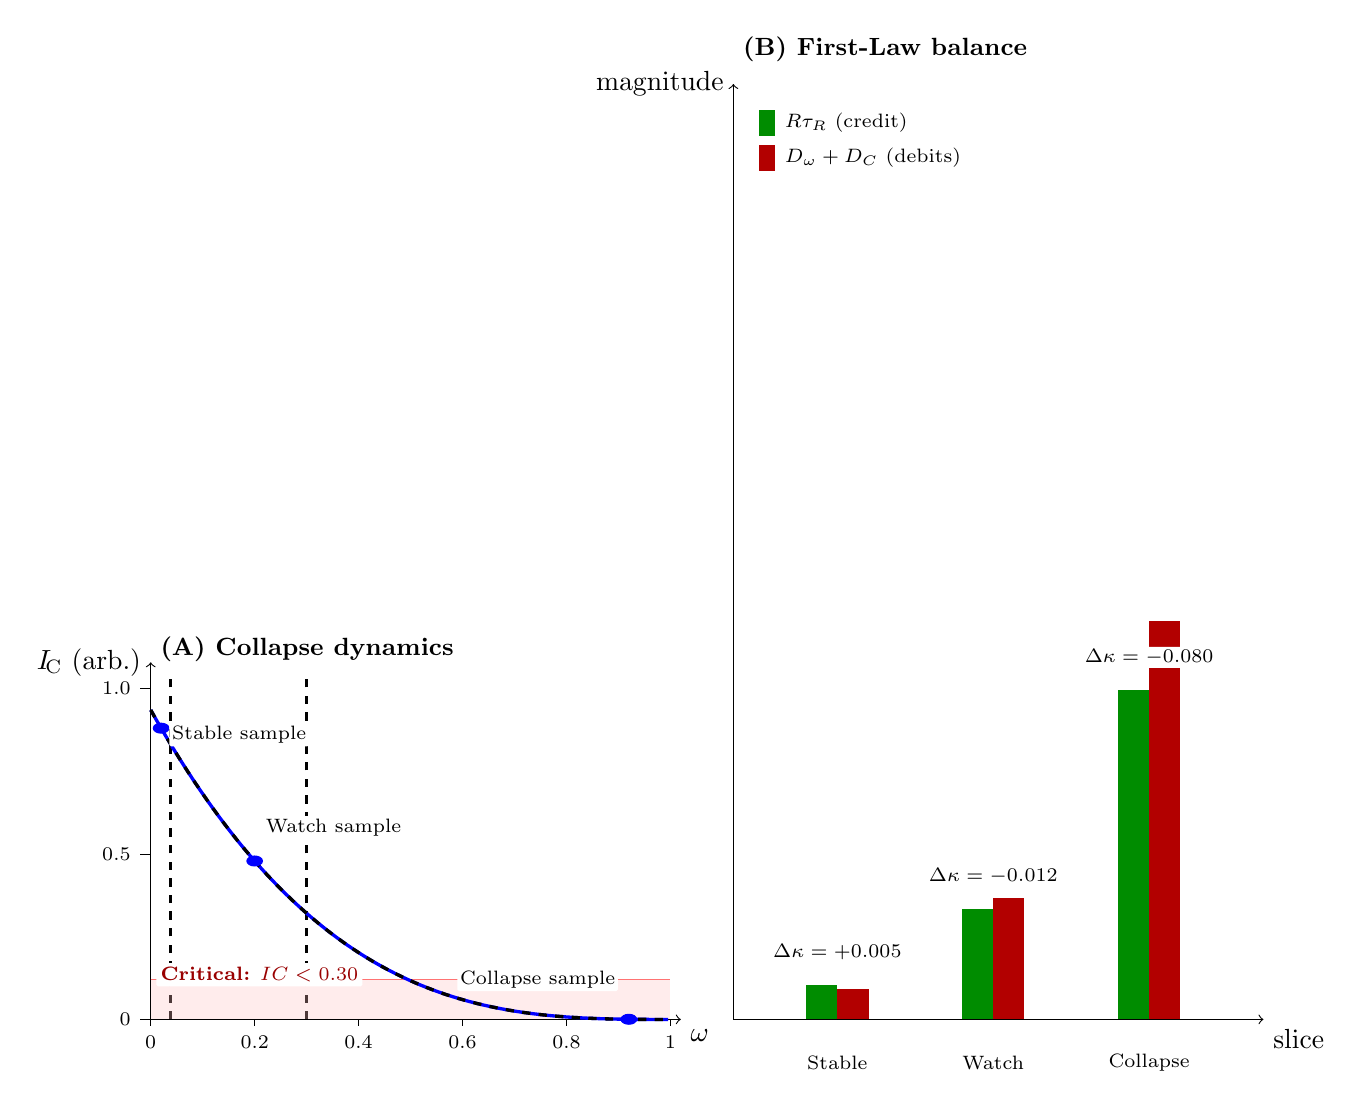
\begin{tikzpicture}

    % Tunables (kept numeric to avoid calc lib):
    % Panel widths in cm (outer scopes below use these as x-scales)
    % Total width ≈ AX + GUT + BX = 6.6 + 0.8 + 6.6 = 14.0 cm (fits textwidth)
    % Heights are set by y-scales.
    % Panel A
    %   x-scale = 6.6cm, y-scale = 4.2cm
    % Panel B
    %   x-scale = 6.6cm, y-scale = 11.0cm
    % Gutter (horizontal gap) = 0.8cm

    %==========================
    % Panel (A): IC vs ω
    %==========================
    \begin{scope}[shift={(0,0)}]
      \begin{scope}[x=6.6cm,y=4.2cm]
        % axes
        \draw[->] (0,0) -- (1.02,0) node[below right] {$\omega$};
        \draw[->] (0,0) -- (0,1.08) node[left] {$I_{\!\mathrm{C}}$ (arb.)};
        % ticks (x)
        \foreach \x/\lbl in {0/0,0.2/0.2,0.4/0.4,0.6/0.6,0.8/0.8,1/1} {
          \draw (\x,0) -- ++(0,-0.02) node[below,font=\scriptsize] {\lbl};
        }
        % ticks (y)
        \foreach \y/\ylbl in {0/0,0.5/0.5,1/1.0} {
          \draw (0,\y) -- ++(-0.02,0) node[left,font=\scriptsize] {\ylbl};
        }

        % Regime thresholds
        \draw[dashed,very thick] (0.038,0) -- (0.038,1.05);
        \draw[dashed,very thick] (0.30,0) -- (0.30,1.05);

        % Critical overlay ribbon
        \fill[red!25,opacity=0.30] (0,0) rectangle (1,0.12);
        \draw[red!55] (0,0.12) -- (1,0.12);
        \node[anchor=west,red!60!black,fill=white,rounded corners=0.6pt,inner sep=1.5pt,font=\scriptsize]
          at (0.01,0.135) {\textbf{Critical:} $IC<0.30$};

        % Curves (α=1, C=0.20, τ_R=2.0, ε=1e-8)
        \draw[very thick,blue,domain=0:0.999,samples=240,smooth,variable=\w]
          plot ({\w},{ (1-\w)*(1-\w) * (1-\w+0.00000001) * exp(-0.2/3.0) });
        \draw[very thick,dashed,domain=0:0.999,samples=240,smooth,variable=\w]
          plot ({\w},{ (1-\w)*(1-\w)*(1-\w) * exp(-0.2/3.0) });

        % Sample markers (Stable, Watch, Collapse)
        \filldraw[blue] (0.02, { (1-0.02)^2*(1-0.02+0.00000001)*exp(-0.2/3.0) }) circle (0.015);
        \node[anchor=west,font=\scriptsize,fill=white,rounded corners=0.6pt,inner sep=1pt]
          at (0.035,0.86) {Stable sample};

        \filldraw[blue] (0.20, { (1-0.20)^2*(1-0.20+0.00000001)*exp(-0.2/3.0) }) circle (0.015);
        \node[anchor=west,font=\scriptsize,fill=white,rounded corners=0.6pt,inner sep=1pt]
          at (0.215,0.58) {Watch sample};

        \filldraw[blue] (0.92, { (1-0.92)^2*(1-0.92+0.00000001)*exp(-0.2/3.0) }) circle (0.015);
        \node[anchor=east,font=\scriptsize,fill=white,rounded corners=0.6pt,inner sep=1pt]
          at (0.90,0.12) {Collapse sample};

        % Panel label
        \node[anchor=west,font=\small\bfseries] at (0,1.12) {(A) Collapse dynamics};
      \end{scope}
    \end{scope}

    %==========================
    % Panel (B): First-Law bars
    %==========================
    % shift = panel A width (6.6cm) + gutter (0.8cm) = 7.4cm
    \begin{scope}[shift={(7.4,0)}]
      \begin{scope}[x=6.6cm,y=11cm] % y-scale so 0.46 ≈ 5.06cm
        % axes
        \draw[->] (0,0) -- (1.02,0) node[below right] {slice};
        \draw[->] (0,0) -- (0,1.08) node[left] {magnitude};

        % x positions for three slices
        \def\xS{0.20}  % Stable
        \def\xW{0.50}  % Watch
        \def\xC{0.80}  % Collapse

        % Heights (Appendix D values)
        \def\RS{0.040} \def\DS{0.035} \def\dKS{0.005}
        \def\RW{0.128} \def\DW{0.140} \def\dKW{-0.012}
        \def\RC{0.380} \def\DC{0.460} \def\dKC{-0.080}

        % Bar width
        \def\bw{0.06}

        % Credits (green) and Debits (red)
        \fill[green!55!black] (\xS-\bw,0) rectangle (\xS, \RS);
        \fill[red!70!black]   (\xS,0)     rectangle (\xS+\bw, \DS);

        \fill[green!55!black] (\xW-\bw,0) rectangle (\xW, \RW);
        \fill[red!70!black]   (\xW,0)     rectangle (\xW+\bw, \DW);

        \fill[green!55!black] (\xC-\bw,0) rectangle (\xC, \RC);
        \fill[red!70!black]   (\xC,0)     rectangle (\xC+\bw, \DC);

        % Slice labels
        \node[font=\scriptsize] at (\xS, -0.05) {Stable};
        \node[font=\scriptsize] at (\xW, -0.05) {Watch};
        \node[font=\scriptsize] at (\xC, -0.05) {Collapse};

        % Δκ annotations
        \node[font=\scriptsize,fill=white,rounded corners=0.6pt,inner sep=1pt]
          at (\xS, \RS+0.038) {$\Delta\kappa=+0.005$};
        \node[font=\scriptsize,fill=white,rounded corners=0.6pt,inner sep=1pt]
          at (\xW, \RW+0.038) {$\Delta\kappa=-0.012$};
        \node[font=\scriptsize,fill=white,rounded corners=0.6pt,inner sep=1pt]
          at (\xC, \RC+0.038) {$\Delta\kappa=-0.080$};

        % Compact legend (top-left)
        \fill[green!55!black] (0.05,1.02) rectangle ++(0.03,0.03);
        \node[anchor=west,font=\scriptsize] at (0.08,1.035) {$R\tau_R$ (credit)};
        \fill[red!70!black] (0.05,0.98) rectangle ++(0.03,0.03);
        \node[anchor=west,font=\scriptsize] at (0.08,0.995) {$D_{\omega}+D_{C}$ (debits)};

        % Panel label
        \node[anchor=west,font=\small\bfseries] at (0,1.12) {(B) First-Law balance};
      \end{scope}
    \end{scope}

  \end{tikzpicture}

  \caption{Collapse dynamics and the First Law. \textbf{(A)} Integrity $I_{\!\mathrm{C}}$ falls rapidly as $\omega\!\uparrow$; regime cuts (dashed) at $\omega=0.038$ and $\omega=0.30$; the shaded ribbon marks the \emph{Critical overlay} ($IC<0.30$). \textbf{(B)} First-Law balance on three slices (same-anchor exemplars): credit $R\tau_R$ (green) vs.\ debits $D_{\omega}{+}D_C$ (red); residuals are zero by construction: Stable $[+0.005]$, Watch $[-0.012]$, Collapse $[-0.080]$. 
  \textbf{Contract}: $(a,b,\varepsilon,p,\alpha)=(-3.7280384,\,10.856631,\,10^{-8},\,3,\,1.0)$. 
  \textbf{Face policy}: \texttt{post\_clip+guard}.}
  \label{fig:collapse-dynamics-firstlaw}
\end{figure}
